\section{ Problem Description and Formulation}
To avoid manual calibration of sensors that often make the system less deployable and to maximize estimation accuracy, we actively take advantage of existing information source, namely the main water meter. This section elaborates ways of fusing two types of information that help each other to improve their spatial granularity and accuracy.  

\begin{figure}
\centering
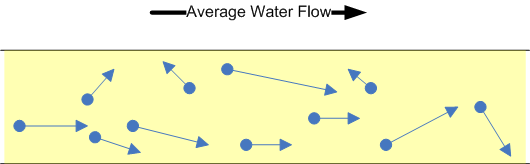
\includegraphics[width=80mm]{.//figures/water.png}
\caption{Microscopic View of Water Flow in a Pipe}
\vskip -6pt
\end{figure}

\subsection{Water Flow Rate Estimation using Vibration Sensors}
To formulate the model of NAWMS, we start with the microscopic view of water flow in a pipe given in [], build up some optimization problems depending on pipe topologies, which minimize performance metric of the system, namely the sum of estimation error.  

\subsubsection{Theory of Operation}
This section describes how vibration on a pipe can be related to water flow rate in a pipe. Looking at water flow in a pipe in a microscopic way, there are many molecules flow toward the flow direction in average. Each molecule has its own velocity as shown in the figure 2. While water is flowing toward its flow direction, many molecules hit the pipe. According to the first law of thermodynamics, some of the kinetic energy is converted to heat as the turbulent eddies dissipate, but most is converted into potential energy in the form of pressure [Pittard 2003]. Evans et. al.p[  showed that the variance of vibration is proportional to the average flow rate in a pipe. The following is a brief excerpt from [Evans] that illustrate the mathematical model of this concept. 

The local velocity at a point can be regarded as superposition of an average velocity and instantaneous fluctuating velocity. The fluid velocities can be decomposed in time averaged velocities and fluctuation velocities. Let define  $u$ be the velocity parallel to the pipe axis and $v$ be the velocity perpendicular to the pipe axis. The instantaneous velocities $u,v$, can be written as a sum of the average velocities $\bar{u},\bar{v}$ and the fluctuation velocities $u',v'$. 
\begin{equation}
\begin{array}{l}
u=\bar{u}+u' \\
v=\bar{v}+v'=v'
\end{array}
\end{equation}
Since there is no net flow in the perpendicular direction to the pipe axis, the time averaged velocity $\bar{v}$is zero. 
Prashun[] showed that the time average of the product of the velocity fluctuation is less than zero. 
\begin{equation}
\overline{u'v'} < 0
\end{equation}
Prashun[] also demonstrated that for a circular conduit of radius $r$, the shear stress $\tau$ at the wall can be related to the pressure $p$ as follows.  
\begin{equation}
\begin{array}{l}
\tau=-\frac{r}{2}\frac{dp}{dx}\\\\
\frac{dp}{dx}=p'=-\frac{2\tau}{r}
\end{array}
\end{equation}
From the Navier-Stokes equations, Prashun[] also demonstrated that for turbulent flow, the turbulent shear stress can be expressed as
\begin{equation}
\tau=-\rho\overline{u'v'}
\end{equation}
Equations [][][] yield that the pressure fluctuation is proportional to the fluctuation of the fluid velocity. 
\begin{equation}
p' \propto \overline{u'v'}
\end{equation}
In addition, it can be shown that the pipe vibration is proportional to the pressure fluctuations in the fluid. First, the fluid filled pipe system can be depicted as a one-dimensional model of a beam. It is well known from structural mechanics that the rate of change of the moment along a beam is equal to the shear and the rate of change of shear, $dV/dx$, along the length of the beam is equal to the pressure fluctuations, $p'(x)$, per unit length as
\begin{equation}
\frac{d^{2}M}{dx^{2}}=\frac{dV}{dx}=p'(x)
\end{equation}

When a beam is subjected to bending, one side of the beam is in tension while the other side is in compression. Differentiating the Flexture Equation () twice with respect to x, then using the relationship for p� gives

\begin{equation}
\begin{array}{l}
M=EI\frac{d^{2}y}{dx^{2}} \\\\ 
\frac{d^{2}M}{dx^{2}}=EI\frac{d^{4}y}{dx^{4}}=p'(x)
\end{array}
\end{equation}

To relate the pressure fluctuations to the pipe acceleration, consider the differential equation of motion for transverse vibration of a beam as given by Seto[]
\begin{equation}
\frac{\partial ^{2}y}{\partial t^{2}}=-\frac{EIg}{A\gamma}\frac{\partial ^{4}y}{\partial x^{4}}
\end{equation}
where

$A$ : cross sectional area of the beam

$\gamma$ : specific weight of the beam

$g$ : gravity

$EI$ : flexural rigidity

Since $A$, $g$, and $\gamma$ are constant, equation () can be rewritten for convenience

\begin{equation}
\frac{\partial ^{2}y}{\partial t^{2}}=-CEI\frac{\partial ^{4}y}{\partial x^{4}}=-Cp'(x)
\end{equation}

where $C=\frac{g}{A\gamma}$

This indicates that the acceleration of the pipe is proportional to the pressure fluctuations in the fluid. The basic theory of operation will be based on the relationship between the standard deviation of the pipe vibrations and the mean flow rate of the fluid in the pipe. Blake[] stated that the generation of vibrations by fluid motion involves the reactions of fluids and solids to stresses imposed by time-varying flow. For dynamically similar flows, the radio of the flow fluctuations to the average flow is constant. Bird et. al.[] showed that this relationship by noting that the oscillatory term is the time average of the absolute magnitude of the oscillation, given by  where  . They defined this as �intensity of turbulence,� which is a measure of the magnitude of the turbulent disturbance, and is given by $\frac{\sqrt{\bar{m}}}{\bar{u}}=$ intensity of turbulence

From the definition of turbulent flow, the intensity of turbulence expression can be rearranged as
\begin{equation}
\frac{\bar{m}}{\bar{u}^{2}}=\frac{\frac{1}{N}\sum_{i=1}^{N}\left[u_{i}(t)-\bar{u}\right]^{2}}{\bar{u}^{2}}
\end{equation}

Multiplying both side by the number of points N and $\bar{u^{2}}$ and dividing by N-1, we get
\begin{equation}
\frac{1}{N-1}\sum_{i=1}^{N}\left[u_{i}(t)-\bar{u}\right]^{2}=\frac{NC}{N-1}\bar{u}^{2}=K\bar{u}^{2}
\end{equation}

This shows the flow fluctuations are proportional to the pressure fluctuations and the pressure fluctuations are proportional to the pipe vibration, it also follows that the standard deviation of the pipe vibrations is proportional to the average flow rate.
This result doesn�t necessarily show that the water flow rate in a pipe is linearly proportional to the vibration on the pipe. Instead they have a non-linear but proportional relation due to non-linear characteristics of vibration sensors, pipe structure, turbulence, etc. Experimental result in section ?? shows this relationship.

\subsubsection{ Vibration to Flow Rate Model}
\begin{figure}
\centering
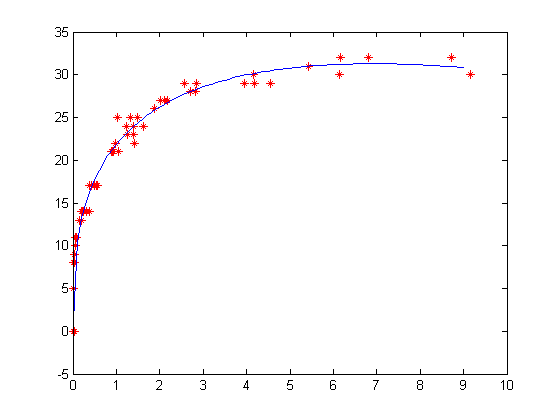
\includegraphics[width=80mm]{.//figures/copper.png}
\caption{Copper Pipe Vibration to Water Flow Rate}
\vskip -6pt
\end{figure}

Although the concept given in section 3.1.1 will be shown in section 4 through elaborate experimental  results, this section briefly introduce the vibration to the flow rate model to formulate a large scale water flow rate monitoring system using less intrusive vibration sensors. To see the relationship between vibration and water flow rate, we measured vibration on a pipe and water flow rate in the pipe while changing water flow rate by changing faucet   valve position. Figure ?? illustrate that water we may fit the curves and the fitted curve equations are as follows,
\begin{equation}
f(t)=\alpha \sqrt[3]{v(t)}+\beta \sqrt{v(t)}+\gamma v(t) + \delta
\end{equation}
where

$f(t)$ : water flow rate

$v(t)$ : vibration

Section 4.? will describe this model gives less error thus is the best and simple form, we took the model for vibration to flow rate relationship to construct the large scale water flow rate monitoring system. 

\subsection{Simple Pipe Structure}
\begin{figure}
\centering
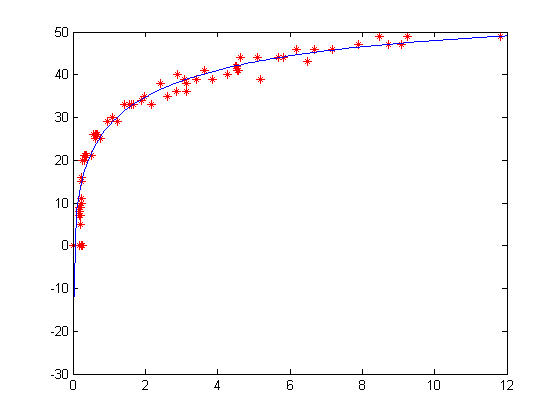
\includegraphics[width=80mm]{.//figures/pvc.png}
\caption{PVC Pipe Vibration to Water Flow Rate}
\vskip -6pt
\end{figure}

\begin{figure}
\centering
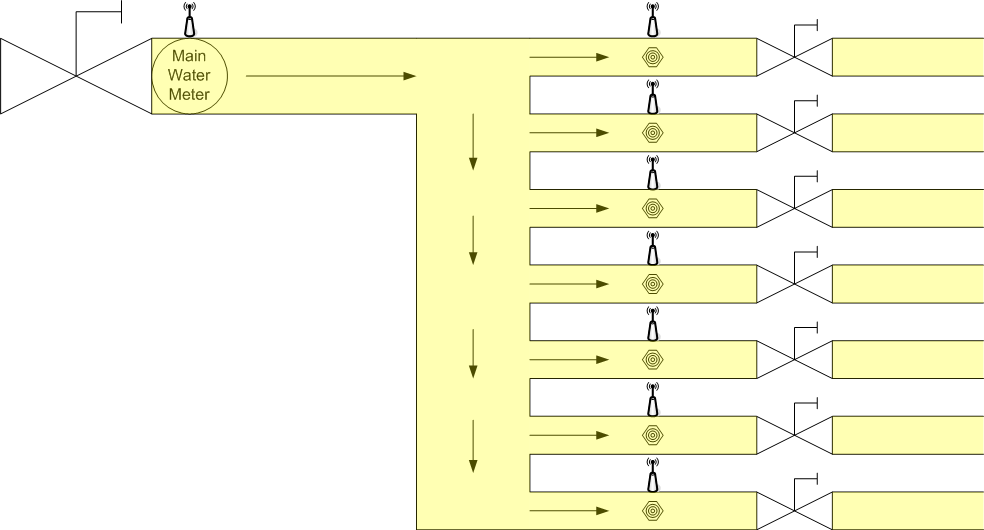
\includegraphics[width=80mm]{.//figures/pipes.png}
\caption{Complex Pipe Topology}
\vskip -6pt
\end{figure}



In this section, we formulate the large scale water flow rate monitoring system that consists of one main water meter, many vibration sensors on pipes, and an aggregation unit. Using the information from the main water meter that is more accurate but lacks spatially finer grained information, the system calibrates parameters (alpha, beta, gamma and delta) of every vibration sensors while solving an optimization problem. This problem can be generalized for more general pipe topologies shown in figure ?? and we will discuss this in the next section. Firstly, consider a simple  pipe topology where one main pipe is equipped with he main water meter and N pipe branches where we put vibration sensors. The main water meter gives us its real-time water flow in the main pipe and let define $M(t)$ as water flow rate of the main pipe. Let define the water flow rate of each branches as $f_{i}(t)$ where $i$ is pipe index number. Since all branches are connected to the main pipe, we can immediately get eq() because the total water flow rate is the sum of all the flow rate in every pipe branches.

\begin{equation}
M(t) = \sum _{i=1} ^{N} f_{i}{(t)}
\end{equation}
where

$N$: Total number of pipes

From section 2, we approximate mapping from variance of vibration on a pipe to actual water flow rate in the pipe as follows,[model validation needed]

\begin{equation}
f_{i}(t)=\alpha_{i} \sqrt[3]{v_{i}(t)}+\beta_{i} \sqrt{v_{i}(t)}+\gamma_{i} v_{i}(t) + \delta_{i}
\end{equation}

According the relationship shown in section 3.1.1, it has to be a linear mapping from the variance of vibration to the flow rate. Due to sensor and pipe saturation and unmodeled parameters as mentioned earlier, we put additional terms to capture these. 

In order to estimate $\alpha_{i}, \beta_{i}, \gamma_{i}$, and $\delta_{i}$ one can calibrate each sensor at a time using a vibration sensor and water flow meter pair, however it requires manual effort that increases installation cost. We want to avoid this to reduce installation by introducing an optimization problem that yields all the parameters.

Assume every sensor samples every $\Delta t$ and every sensor is synchronized. Consider equation () and we get $M(\Delta kt) = \sum_{i=1}^{N} f_{i}(\Delta kt)$

After getting M samples, we get $\sum_{k=1}^{M}M(\Delta kt) = \sum_{k=1}^{M}\sum_{i=1}^{N} f_{i}(\Delta kt)$ 

Since we know this equality always holds unless there is water leakage, we can formulate this as an optimization problem as follows
\begin{equation}
\begin{array}{ccc}
min &&\left|\left|\sum_{k=1}^{M}M(\Delta tk) - \sum_{k=1}^{M}\sum_{i=1}^{N} f_{i}(\Delta tk)\right|\right|_{1}\\\\
subject & to & \\\\
&&
0 \leq f_{i}(\Delta tk) \leq f_{i},max 
\end{array} 
\end{equation}
where

$f_{i}(\Delta tk)=\alpha_{i}\sqrt[3]{v_{i}(\Delta tk)}+\beta_{i}\sqrt{v_{i}(\Delta tk)}+\gamma_{i}v_{i}(\Delta tk)+\delta_{i} $

$\Delta t$ : Sampling Time 

$M$ : Number of Samples

$N$ : Number of Pipes
\\


Solving this optimization problem yields all the necessary parameters if it gives the global optimum and is only one point. This equation also implies that for the calibration no human intervention is needed as the optimization and sampling can be automated. Note that, this optimization problem consists only of linear constraints and its objective function can be also formulated as a linear objective function[]. Therefore, any available LP solver can solve this problem very efficiently and guarantees global optimum.

\subsection{General Pipe Structure}
\begin{figure}
\centering
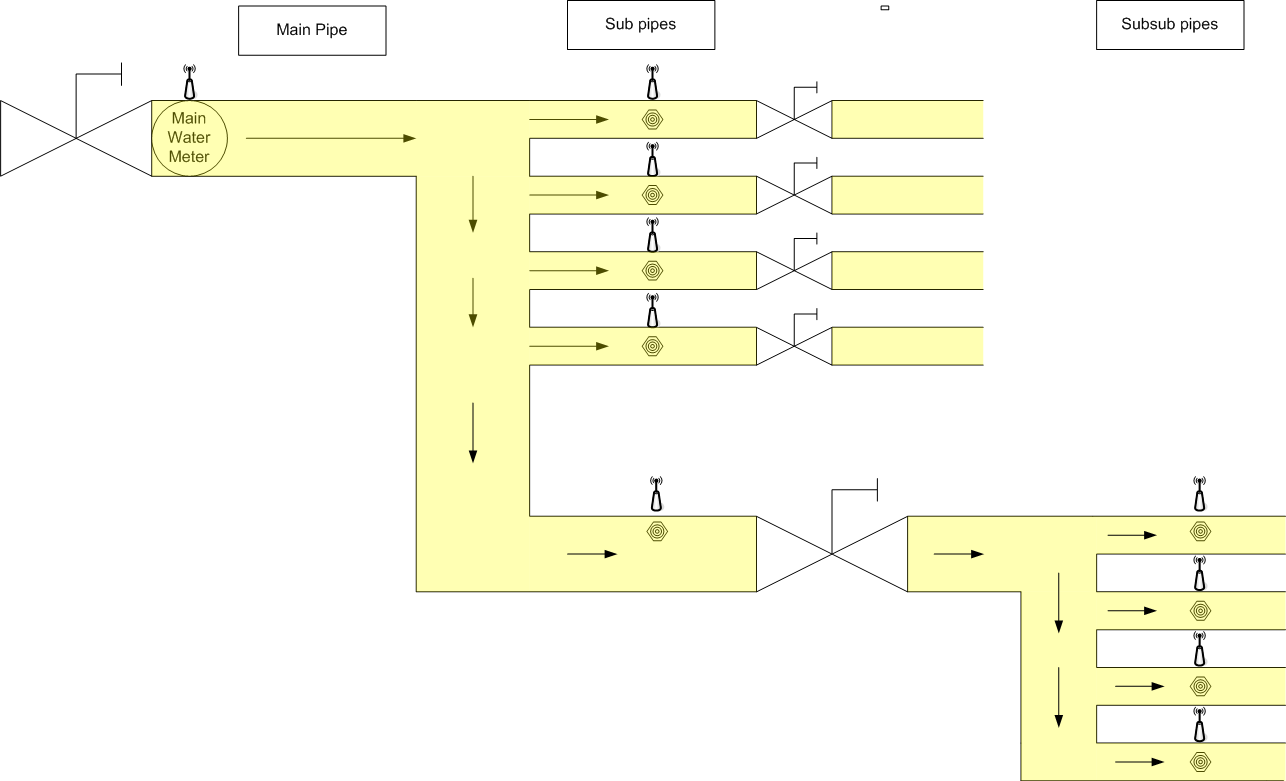
\includegraphics[width=80mm]{.//figures/pipes2.png}
\caption{Complex Pipe Topology}
\vskip -6pt
\end{figure}

Since this optimization problem minimizes the error; (Total Water Flow Rate - Sum of Water Flow Rate of every pipe branches), it guarantees minimum error in its estimation. However section 3.2 only considers one simple pipe topology, in this section we consider a more general topology of pipe structure and show that the problem can be decomposed depending on their topology. This might have more than one optimization problem but can be solved very efficiently in known polynomial time. Thus, we describes how to decompose a more complex topology of the pipes but rest of the paper focuses on the first problem() as each of optimization problem can be dealt with separately.  
Consider a pipe structure in figure ??, assuming there is no water leakage, the total flow rate must be the sum of water flow rate of sub pipes. Similarly the flow rate of each sub pipe must be the sum of flow rate of its sub-sub pipes. Therefore we have K equalities that need to hold to satisfy the law of mass conservation. 
Let define the water flow rate in a pipe as 
$f_{i,j}(t)$ where $i$ is sub pipe index and $j$ is sub-sub pipe index

Due to the law of mass conservation, these two equations must hold unless there's water leakage in a pipe
\begin{equation}
\begin{array}{l}
f_{i}(t) = \sum_{j=1}^{J}f_{i,j}(t)\\
 M(t) = \sum_{i=1}^{N}f_{i}(t)
\end{array}
\end{equation}
\\

From the equations () and (), we can immediately get the following which is a slight modification of equation (). 

\begin{equation}
\begin{array}{ccc}
min &&\left|\left|\sum_{k=1}^{M}M(\Delta tk) - \sum_{k=1}^{M}\sum_{i=1}^{N} f_{i}(\Delta tk)\right|\right|_{1}\\\\
subject & to & \\\\
&&
0 \leq f_{i}(\Delta tk) \leq f_{i},max \\\\
&& f_{i}(\Delta kt) = \sum_{j=1}^{J_{i}}f_{i,j}(\Delta kt)
\end{array} 
\end{equation} 
where

$f_{i}(\Delta tk)=\alpha_{i}\sqrt[3]{v_{i}(\Delta tk)}+\beta_{i}\sqrt{v_{i}(\Delta tk)}+\gamma_{i}v_{i}(\Delta tk)+\delta_{i} $

$\Delta t$ : Sampling Time

$M$ : Number of Samples

$N$ : Number of Pipes 

$J_{i}$ : Number of sub-pipe branches of i-th sub-pipe of the main pipe
\\


Similarly, this concept can be generalized as the main pipe water flow rate is the sum of its sub pipe branches, a sub pipe branch flow rate is the sum of its sub-sub pipe branches and so forth. 
Therefore, depending on users� need, one can always make these equalities to formulate similar problem forms. For example, if they are interested in the water flow rate to the bathroom rather than each of bathroom sink, toilet bin, and  shower booth, they want to omit individual pipe, instead they want to monitor a sub pipe that has each of branches. 
 
 \subsection{Account for Vibration Propagation}

 \begin{figure}
\centering
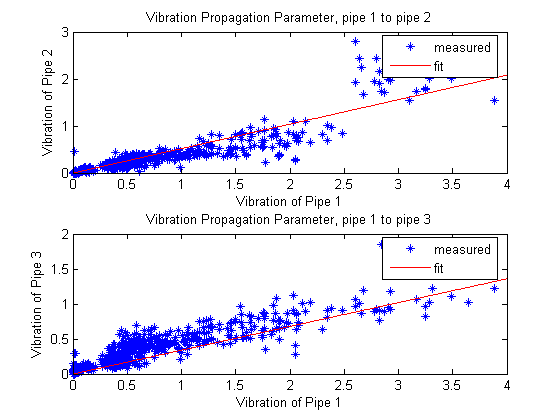
\includegraphics[width=80mm]{.//figures/P123.png}
\caption{Vibration Propagation from Pipe 1 to Pipe 2 and Pipe 3}
\vskip -6pt
\end{figure}

 \begin{figure}
\centering
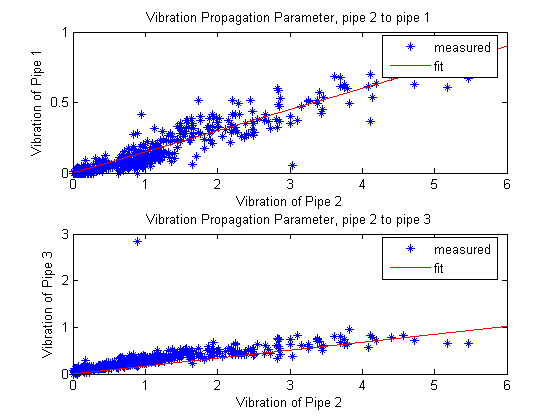
\includegraphics[width=80mm]{.//figures/P213.png}
\caption{Vibration Propagation from Pipe 2 to Pipe 1 and Pipe 3}
\vskip -6pt
\end{figure}

 If we consider a pipe structure in figures ?? and ??, we didn�t take vibration propagation among pipes into account. However, pipes are physically connected and metal and PVC pipes are pretty good material that transfer vibration among themselves. Therefore, the model needs to consider vibration propagation among pipes and compensate this effect to achieve better precision. 
In general, the vibration propagation may not be linear because pipe topology could be very complex, connection among pipes may consist of hybrid material, different types of mechanical structure have different resonance frequency, etc. Since the water flow induced vibration if relatively small, we want to assume that the vibration propagation is linear and show this through our experiment in section 4.??. 
Consider there is vibration only on pipe j and let first define propagation parameter from pipe i to pipe j as
 
 \begin{equation}
 v_{m,i}(t) = p_{i,j}v_{j}(t)
 \end{equation}
 
 where
 
 $v_{m,i}(t)$ : measured vibration on pipe i
 
 $p_{i,j}$ : Vibration Propagation Constant from pipe j to pipe i
 
 $v_{j}(t$ : Water Flow induced Vibration on pipe j
\\

Since we see this vibration is linear, the measured vibration on the pipe i is the superposition of all possible vibrations from pipe 1 to N as follows

\begin{equation}
v_{m,i}(t) = \sum_{j=1}^{N}p_{i,j}v_{j}(t)
\end{equation}
where

$v_{m,i}(t)$ : Measured Vibration on pipe i
$p_{i,j}$ : Vibration Propagation Coefficient
$v_{j}(t)$ : : Water Flow induced Vibration on pipe j

Note also that, 

$p_{i,j} = 1$  if $i=j$

$0 \leq p_{i,j} \leq 1$ otherwise

Because the pipe architecture is passive, its propagation coefficient cannot exceed 1 and cannot be less than zero.  Once we model this, we can immediately get the following optimization problem by modifying the problem () in section 3. 

\begin{equation}
\begin{array}{ccc}
min &&\left|\left|\sum_{k=1}^{M}M(\Delta tk) - \sum_{k=1}^{M}\sum_{i=1}^{N} f_{i}(\Delta tk)\right|\right|_{1}\\\\
subject & to & \\\\
&&
0 \leq f_{i}(\Delta tk) \leq f_{i},max \\\\
&&v_{m,i}(t) = \sum_{j=1}^{N}p_{i,j}v_{j}(t) \\\\
\end{array} 
\end{equation}

where 

$\Delta t$ : Sampling Time

$M$ : Number of Samples

$N$ : Number of Pipes
\\

Because of propagation effect that adds one posynomial equality constraint, this problem becomes a nonlinear and non-convex optimization problem that is extremely hard to solve. However, we explore two methods of reformulating the problem either as a generalized geometric programming  problem by relaxing and restricting constraints with reasonably tight bound while conserving physical meaning of the problem or as a two phase linear programming problem by decomposing the optimization problem into two problems. It is well known that both geometric programming and linear programming problems can be solved in polynomial time. The following two subsections describe the GP modeling of the problem and the two phase LP modeling and show that one can solve these.
Depending on the system performance and its characteristics, the system can select either one of both optimization problems to achieve its desired accuracy.

\subsection{ Geometric Programming Modeling}
The posynomial equality constraint prevents us to solve the optimization problem as a geometric programming. In addition, the objective function is not a standard geometric programming form. 
\begin{equation}
v_{m,i}(t) = \sum_{j=1}^{N}p_{i,j}v_{j}(t)
\end{equation}

Therefore, we need to reformulate this optimization problem because this problem is in general NP-hard. In this section we describe a derivation of this non-convex optimization to a convex optimization problem with careful modification while maintaining physical meaning of the optimization problem. 
First, we introduce a slack variable s and the problem can be equivalently reformulated as follows,

\begin{equation}
\begin{array}{ccc}
min && s \\\\
subject & to & \\\\
&& -s \leq \sum_{k=1}^{M}\sum_{i=1}^{N} f_{i}(\Delta tk) - \sum_{k=1}^{M}M(\Delta tk)  \leq s\\\\
&&
0 \leq f_{i}(\Delta tk) \leq f_{i},max \\\\
&&v_{m,i}(t) = \sum_{j=1}^{N}p_{i,j}v_{j}(t) 
\end{array} 
\end{equation}

By restricting the original objective function as follows,
\begin{equation}
0 \leq \sum_{k=1}^{M}\sum_{i=1}^{N} f_{i}(\Delta tk) - \sum_{k=1}^{M}M(\Delta tk)  \leq s
\end{equation}

Therefore, we can obtain the following,
\begin{equation}
\begin{array}{ccc}
min && s \\\\
subject & to & \\\\
&& 0 \leq \sum_{k=1}^{M}\sum_{i=1}^{N} f_{i}(\Delta tk) - \sum_{k=1}^{M}M(\Delta tk)  \leq s\\\\
&&
0 \leq f_{i}(\Delta tk) \leq f_{i},max \\\\
&&v_{m,i}(t) = \sum_{j=1}^{N}p_{i,j}v_{j}(t)
\end{array} 
\end{equation}

Now, according to [GP COMM], by relaxing the posynomial equality constraint as an inequality with reasonable tightness, one can reformulate the constraint as a standard geometric programming form. The following relaxation is reasonable as the measured variance of vibration on a pipe is not only the superposition of all the propagated vibration but also from the external vibration source. 

\begin{equation}
\sum_{j=1}^{N}p_{i,j}v_{j}(t) \leq v_{m,i}(t)
 \end{equation}
 As a consequence, we can obtain the following optimization problem, 
 
 \begin{equation}
 \begin{array}{ccc}
min && s \\\\
subject & to & \\\\
&& \sum_{k=1}^{M}\sum_{i=1}^{N} f_{i}(\Delta tk)  \leq s + \sum_{k=1}^{M}M(\Delta tk)\\\\
&&
0 \leq f_{i}(\Delta tk) \leq f_{i},max \\\\
&&  \sum_{j=1}^{N}p_{i,j}v_{j}(t) \leq v_{m,i}(t)
\end{array} 
\end{equation}

where

$f_{i}(\Delta tk)=\alpha_{i}\sqrt[3]{v_{i}(\Delta tk)}+\beta_{i}\sqrt{v_{i}(\Delta tk)}+\gamma_{i}v_{i}(\Delta tk)+\delta_{i} $
\\

According to [GP TUTORIAL] in section 7.3, it is a mixed linear geometric programing, as equation() is a posynomial because eq() is posynomial.

equation () is posynomial as all the alphas, betas, gammas and deltas are positive, and vibration is always positive.
and the sum of posynomials is also a posynomial and because variance is positive by its nature. 
Therefore, one can solve this problem very efficiently (polynomial time) and guarantees the global optimum as it turns out to be a convex programming problem[]. However, this might render a poor solution as we relaxed the constraint although it is reasonable relaxation. Therefore, we also want to introduce two phase Linear Programming program in case it render a poor solution so that the system can select one

\subsection{ Two phase Linear Programming Modeling}
While section 3.5 gives us a convex optimization problem that gives a set of parameters needed for estimating water flow rate in a pipe, one can further reduce its computational complexity if we derive this as an approximate Linear Programming problem. Although propagation parameters are unknown, since pipe topology is static and not changing over time, one can measure propagation parameters in its initial stage. Then ? are constant and can be estimated.
Once propagation parameters are estimated, ? can be obtained thus its posynomial equality term becomes a linear equation. Therefore, the problem can be decomposed into two problems; a) propagation parameter estimation problem and b) water flow rate function coefficient estimation problem. 
\subsubsection{Vibration Propagation Parameter Estimation}
As it is possible to have situation where only one pipe is on at a time during a long period of time, the system can measure vibration on every pipe and water flow happens on a single pipe j. The measured vibration on the pipe j and the water flow induced vibration on the pipe j is the same, thus we get
$v_{m,j}=v_{j}$

Therefore, measured vibration on each of pipe can be expressed as follows

$v_{m,i} = p_{i,j}v_{m,j}$

It is also obvious that 

$p_{i,j}=1$ if $i=j$

$p_{i,j} = \frac{v_{m,i}}{v_{m,j}}$ otherwise

If the system is ideal, the measurement is perfect, and the system model is flawless, then the propagation parameter estimation is trivial as shown above. However, as most of parameter estimation problem relies on some estimation procedure such as least square estimation, 1-norm minimization approach, or infinity-norm minimization approach due to measurement noise, we also need to formulate this as an parameter estimation problem because the system model, sensors and environment are not ideal thus have measurement noise and unmodeled uncertainties. We want to set the problem as a 1-norm minimization problem with some linear inequality constraints as it is less sensitive to the significant outlier than least square problems and this is mainly because cheap sensors and many wireless sensor nodes often suffer from significant outliers and faulty sensor reading[][][]. We can solve this problem using standard LP solvers and also can easily handle linear inequality constraints.

Let define $l$ be a index of sample and $L$ be the total number of samples.
\begin{equation}
\begin{array}{ccc}
min &&\left|\left| \sum_{l=1}^{L}v_{m,i}(l) - \sum_{l=1}^{L}p_{i,j}v_{m,j}(l)\right|\right|_{1}\\\\
subject & to & \\\\
  && 0 \leq p_{i,j} \leq 1 \\
&&p_{i,i} = 1
\end{array} 
\end{equation}


\subsubsection{ Vibration Parameter Estimation}
After getting vibration propagation parameters, the problem simply becomes a typical linear programming problem as a matrix P is invertible. Therefore, we get
\begin{equation}
\begin{array}{ccc}
min &&\left|\left|\sum_{k=1}^{M}M(\Delta tk) - \sum_{k=1}^{M}\sum_{i=1}^{N} f_{i}(\Delta tk)\right|\right|_{1}\\\\
subject & to & \\\\
&&
0 \leq f_{i}(\Delta tk) \leq f_{i},max \\\\
&&V(t) = P^{-1}V_{m}(t)
\end{array} 
\end{equation}
where

$P = [ p_{i,j} ] $

$V(t) = [v_{i}(t)] \in R_{+}^{N} $

$V_{m}(t) = [v_{m,i}(t)] \in R_{+}^{N}$

$\Delta t$ : Sampling Time 

$M$ : Number of Samples

$N$ : Number of Pipes 
\\

So, this form is again a linear programming problem thus one can solve this problem and get parameters. 

\subsection{Correction Mechanism and Performance Index}
By solving the optimization problems given in section, the system can get all the necessary parameters $\{\alpha_{i}, \beta_{i}, \gamma_{i}, \delta_{i}\}$, which map the vibration to the water flow rate as shown in equation (). However, the system characteristics can change over time due to slight topological changes, seasonal temperature changes, or aging effect. In addition, unpredicted turbulence in a pipe, external vibration, etc. can make the estimate less accurate. To compensate these, the system also takes advantage of the water flow rate from the main pipe; 1) it normalizes the overall flow rate based on the total water flow rate in the main pipe, 2) it also updates parameters based on a performance index. 
Considering the water flow rate is the same as the sum of the water flow rate of every branch of the main pipe. We normalize the water flow rate estimate as follows

\begin{equation}
f_{i}(t) = \frac{\hat{f_{i}}(t)M(t)}{\sum_{i=1}^{N}\hat{f_{i}}(t)}
\end{equation}

where

$\hat{f_{i}}(t)$ : Water Flow Rate Estimate

$f_{i}(t)$ : Normalized Water Flow Rate

This normalization can guarantees that the sum of the water flow rate estimate as well as the sum of the accumulated water usage estimate is the same as the true water flow rate and accumulated water usage. But it normalization may add small error to the water flow rate estimate.

Although the normalization gives the bound for the sum of water flow rate estimate, performance of the system can be degraded over time. Since we tried to minimize the sum of estimation error, performance index of the system can be as follows

\begin{equation}
\left| \frac{\sum_{i=1}^{N}\hat{f_{i}}(t)-M(t)}{M(t)} \right|
\end{equation}

It is obvious that if the performance index is around zero it is performing well, otherwise it needs to be recalibrated. 

\subsection{Algorithm Description}
As we formulated some optimization problems, this section describes how the system works from the beginning. Users need to attach sensors on pipes of interest and they also need to specify the topology of the pipes where they put the sensors based on their desire. Figure ?? shows the procedure the system follows. At its initial deployment stage, it gathers vibration and water flow rate data until it get enough data. Then, it solves two optimization problems shown in section ?? and ??. Given the parameters, it starts to estimate water flow rate based on vibration and compare these with the performance. If the performance index is good, it just continues. Otherwise, it recalibrate the sensors. 
\begin{figure}
\centering
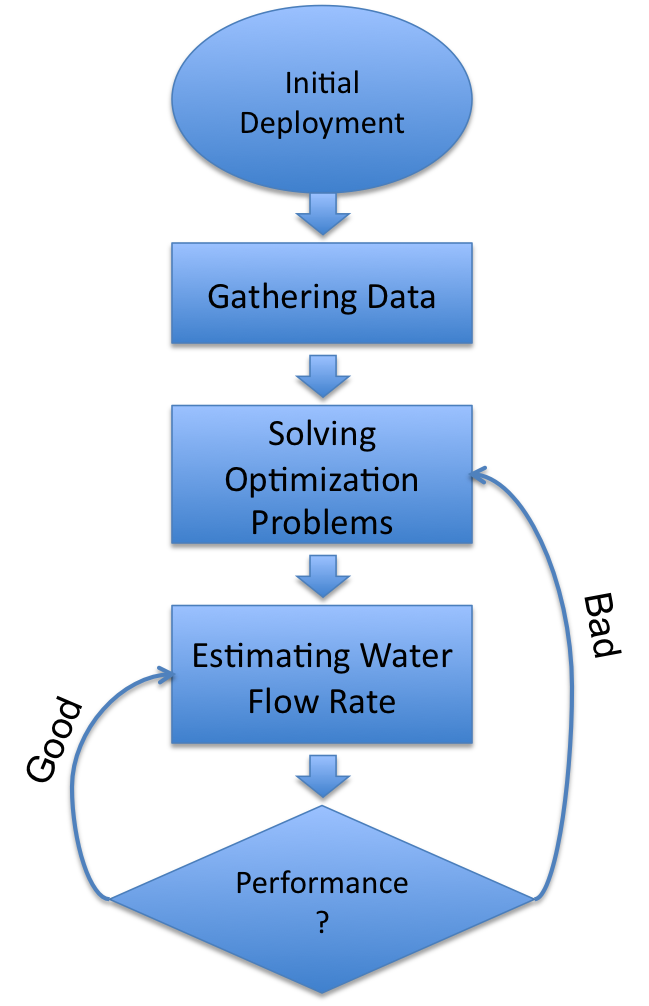
\includegraphics[width=80mm]{.//figures/FlowChart.png}
\caption{Software Flowchart}
\vskip -6pt
\end{figure}

